%% LyX 2.3.4.4 created this file.  For more info, see http://www.lyx.org/.
%% Do not edit unless you really know what you are doing.
\documentclass[12pt,german,journal=mamobx,manuscript=article,maxauthors=15,biblabel=plain]{article}
\usepackage[T1]{fontenc}
\usepackage[latin9]{inputenc}
\usepackage[a4paper]{geometry}
\geometry{verbose,tmargin=1in,bmargin=1in,lmargin=1in,rmargin=1in,headheight=0.5cm,headsep=0.5cm,footskip=0.5cm}
\setlength{\parskip}{\smallskipamount}
\setlength{\parindent}{0pt}
\usepackage{amsmath}
\usepackage{amssymb}
\usepackage{graphicx}

\makeatletter
%%%%%%%%%%%%%%%%%%%%%%%%%%%%%% User specified LaTeX commands.
\usepackage{babel}

\makeatother

\usepackage{babel}
\begin{document}

\section*{�bung 4}

\subsubsection*{Das Bindungs-Fluktuations Modell (Bond Fluctuation Model)}

Mit diesem �bungsblatt verwenden Sie zum ersten Mal das sogenannte
``Bindungs-Fluktuations-Modell'' (BFM), das in der Polymerphysik
h�ufig zur Simulation von Schmelzen und L�sungen verwendet wird. Die
tats�chliche Struktur (Valenzwinkel, Rotationsbarrieren) eines amorphen
Polymers kann f�r eine ausreichende Zahl an Monomeren vernachl�ssigt
werden, so dass sich die statistischen Segmente bis auf das ausgeschlossene
Volumen hin frei zueinander einstellen k�nnen:

\begin{center}
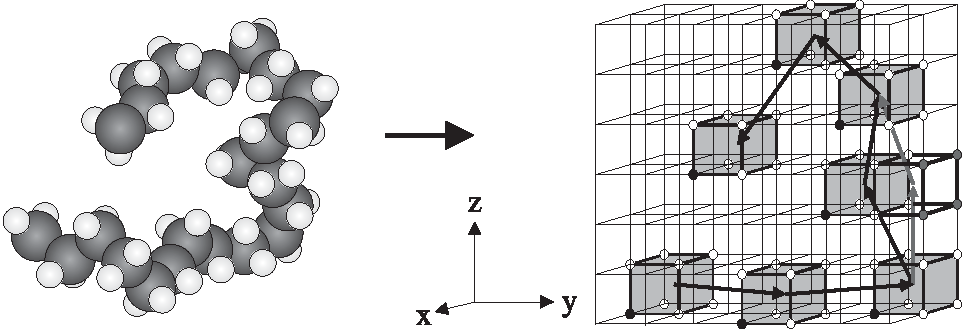
\includegraphics[width=0.9\textwidth]{Abb_3_1} 
\par\end{center}

Die Bindungsvektoren werden auf die Menge $B$

\[
B=P\pm\left(\begin{array}{c}
2\\
0\\
0
\end{array}\right)\bigcup P\pm\left(\begin{array}{c}
2\\
1\\
0
\end{array}\right)\bigcup P\pm\left(\begin{array}{c}
2\\
1\\
1
\end{array}\right)\bigcup P\pm\left(\begin{array}{c}
2\\
2\\
1
\end{array}\right)\bigcup P\pm\left(\begin{array}{c}
3\\
0\\
0
\end{array}\right)\bigcup P\pm\left(\begin{array}{c}
3\\
1\\
0
\end{array}\right)
\]

aus 108 Bindungsvektoren zwischen den Monomeren eingeschr�nkt, um
eine �berkreuzung der Ketten bei einer Bewegung eines Monomers zu
verhindern. $P\pm$ bezeichnet dabei die Menge aller m�glichen Permutationen
und Vorzeichenkombinationen der Vektorkoordinaten. Auf diese Weise
sind 87 verschiedene Winkeleinstellungen zwischen den Segmenten und
f�nf Bindungsl�ngen ($2$, $\sqrt{5}$, $\sqrt{6}$, 3 und $\sqrt{10}$)
m�glich. Die BFM ist damit weitaus flexibler als das bisher eingesetzte
Gittermodell (�bung 3) zur Simulation von Makromolek�len.

Die Bewegung eines Monomers wird folgenderma�en realisiert: Zun�chst
werden statistisch ein Monomer und eine der 6 Bewegungsrichtungen
ausgew�hlt. Anschlie�end wird �berpr�ft, ob f�r die neue Position
des Monomers die Bindungsvektoren zu den Kettennachbarn in $B$ enthalten
sind und ob die 4 Gitterpl�tze in Bewegungsrichtung noch frei sind
(im Falle energetischer Wechselwirkungen w�rde noch der Metropolis-Algorithmus
angewandt). Nur wenn diese Kriterien alle erf�llt sind, wird die Bewegung
durchgef�hrt. Obige Abbildung zeigt einen Sprungversuch in positive
y-Richtung, bei dem alle Voraussetzungen erf�llt sind.

\newpage{}

\subsubsection*{Umsetzung des Bindungs-Fluktuations Modell}

Zur Implementierung des BFM in einer objektorientierten Programmiersprache
erstellen wir zun�chst einzelne Programmteile, mit denen die einzelenen
Bestandteile des Modells umgesetzt werden. Dazu nutzen wir eine Klasse,
die die Positionen der Monomere, ihre Bindungen und ihre Attribute
bereitstellt. Das Bindungsvektorset wird ebenfalls als separate Klasse
implementiert. Das ausgeschlossene Volumen, also das Verbot, dass
ein Gitterplatz von mehreren BFM Einheiten belegt werden kann, wird
�ber ein Gitter und entsprechende Zugriffsfunktionen darauf in einer
eigenen Klasse angelegt. Mit diesen drei Programmbausteinen wird ein
Simulationsobjekt erstellt, mit dem eine Monte-Carlo Bewegung auf
Richtigkeit �berpr�ft und gegebenenfalls ausgef�hrt wird. Eine m�gliche
Realisierung finden Sie in der Datein bfm.py als Python Modul.
\begin{enumerate}
\item Nutzen Sie das gegebene Programm oder eines Ihrer Wahl zur Erstellung
einer einzelnen Polymerkette mit $N=32$ Monomeren.
\item Implementieren Sie die Berechnung des End-zu-End Abstands $R_{\text{ee}}$
und des Gyrationsradius $R_{\text{g}}$.
\item F�hren Sie eine gro�e Anzahl an Simulationen durch ($\approx1000$)
und berechnen Sie damit die Autokorrelationsfunktion des End-zu-End
Vektors $\vec{R}_{\text{ee}}$.
\end{enumerate}

\subsubsection*{Polymer in eingeschr�nkter Geometrie}
\begin{enumerate}
\item Erstellen Sie mit einem geeigneten Programm eine einzelne Polymerkette
mit und ohne ausgeschlossenem Volumem mit $N=64$ in einem Spalt der
Breite $D_{S}$ und einer Pore mit quadratischem Querschnitt der Fl�che
$D_{P}^{2}$ mit verschiedenen Abmessungen. Beobachten Sie den �bergang
von ungest�rten Konformationen zu quasi zwei- bzw. ein-dimensionalen
Konformationen anhand der Ver�nderung des End-zu-End Abstandes und
des Gyrationsradius. Nutzen Sie daf�r die Analyzer aus der letzten
�bung und den UpdaterAddLinearChains aus dem LeMonADE-repository.
\item Erstellen Sie einen Analyzer zur Berechnung der Paarkorrelationsfunktion
$g(r)$ (radiale Verteilungsfunktion):
\[
g(r)=\frac{V}{N^{2}}\langle\sum_{j\neq i}^{N}\delta(r-|R_{\text{i}}-R_{\text{j}}|)\rangle
\]
mit der Teilchenzahl $N$ und den Monomerpositionen $\vec{R}_{i,j}$.
Welche Informationen k�nnen Sie $g(r)$ entnehmen? Welche Gr��en lassen
sich daraus ableiten?
\end{enumerate}

\end{document}
